Space allocation of the subsystems described in the previous section, as well as crew members, is performed with the goals of:
\begin{itemize}
\item Accommodating subsystems necessary to support interplanetary flight and entry
\item Providing crew members with a habitable volume and operational items to support a flight duration of approximately 100 days
\item Keeping the axial position of the \gls{cg} forward to lower pitch stability and alleviate pitch control performance in the final mission phase
\item Allowing for packaging freedom in achieving a static lateral \gls{cg} offset for creating an asymmetric lifting shape
\end{itemize}
To this end, the crew module is packaged as depicted in Figures \ref{fig:axview} and \ref{fig:topview}. 

The top part is required to contain drogues to stabilize the entry vehicle in its final descent phase. Four drogues are placed to incorporate redundancy and provide
a symmetric configuration, to prevent excessive tilting during final descent. Moreover, the top part contains the foldable solar arrays required to generate power required during interplanetary transfer. These are placed in the top part to prevent interference with the flow during entry on one hand and with thrusters and the stowed inflatable before entry on the other hand. A high-gain antenna of adjustable attitude on a boom enables communication during all mission phases. A first-order estimate for the length of this upper part is $0.2$ $[m]$, based on the Orion configuration\footnote{URL:\url{http://www.spaceflight101.com/orion-spacecraft-overview.html}. Accessed: 15-06-2015}.

Crew members are located in the next part, a habitable volume to their availability that is dictated by the performance limit for a three-month mission duration as 11 $[m^{3}]$ per crew member \cite{Rudisill2008}. The diameter of the habitable volume is 4.0 $[m]$, thereby less than vehicle maximum diameter to accommodate four propellant tanks, one per quadrant, that allow intertank propellant transfer to shift the lateral \gls{cg} position. The tanks are sized on the basis of the total required propellant and provide propellant for both the reaction control thrusters and main thruster. The length of this part follows from the habitable volume and depends on the number of crew members.

Operational items are located below, within reach of crew members. These are placed at this location because of their relatively high mass and therefore contribution to the axial \gls{cg} position. The total volume occupied follows from Table \ref{tab:crewmemberops}. On one hand these operational items include relatively dense products, foremostly the life support systems, and less dense products in the form of food and other supplies. Arranging these items asymmetrically allows for a lateral \gls{cg} offset, most notably considering the depleted supplies of food at the end of interplanetary transfer while life support system mass remains intact. The length of this part follows from the required volume for operational items.

The last part of the crew module contains four struts for touchdown, packed symmetrically. The struts are arranged about the batteries required to provide power during entry, where solar panels are stowed, a nitrogen tank for inflation of the inflatable aeroshell and the main thruster to provide in-plane velocity changes. The length follows from estimates for the strut required volume based on the Apollo landers and is an estimated 1.0 $[m]$. 

The last part contains the thruster nozzle, closed off by a heat-resistant end-cap during entry, and the attachment rings for the inflatable decelerator. It is detachable from the main body and thereby does not contain any other subsystems. The length of this part is mainly dictated by the shape of the inflatable and where it attaches to the centerbody.

\begin{figure}[h]
		\centering
		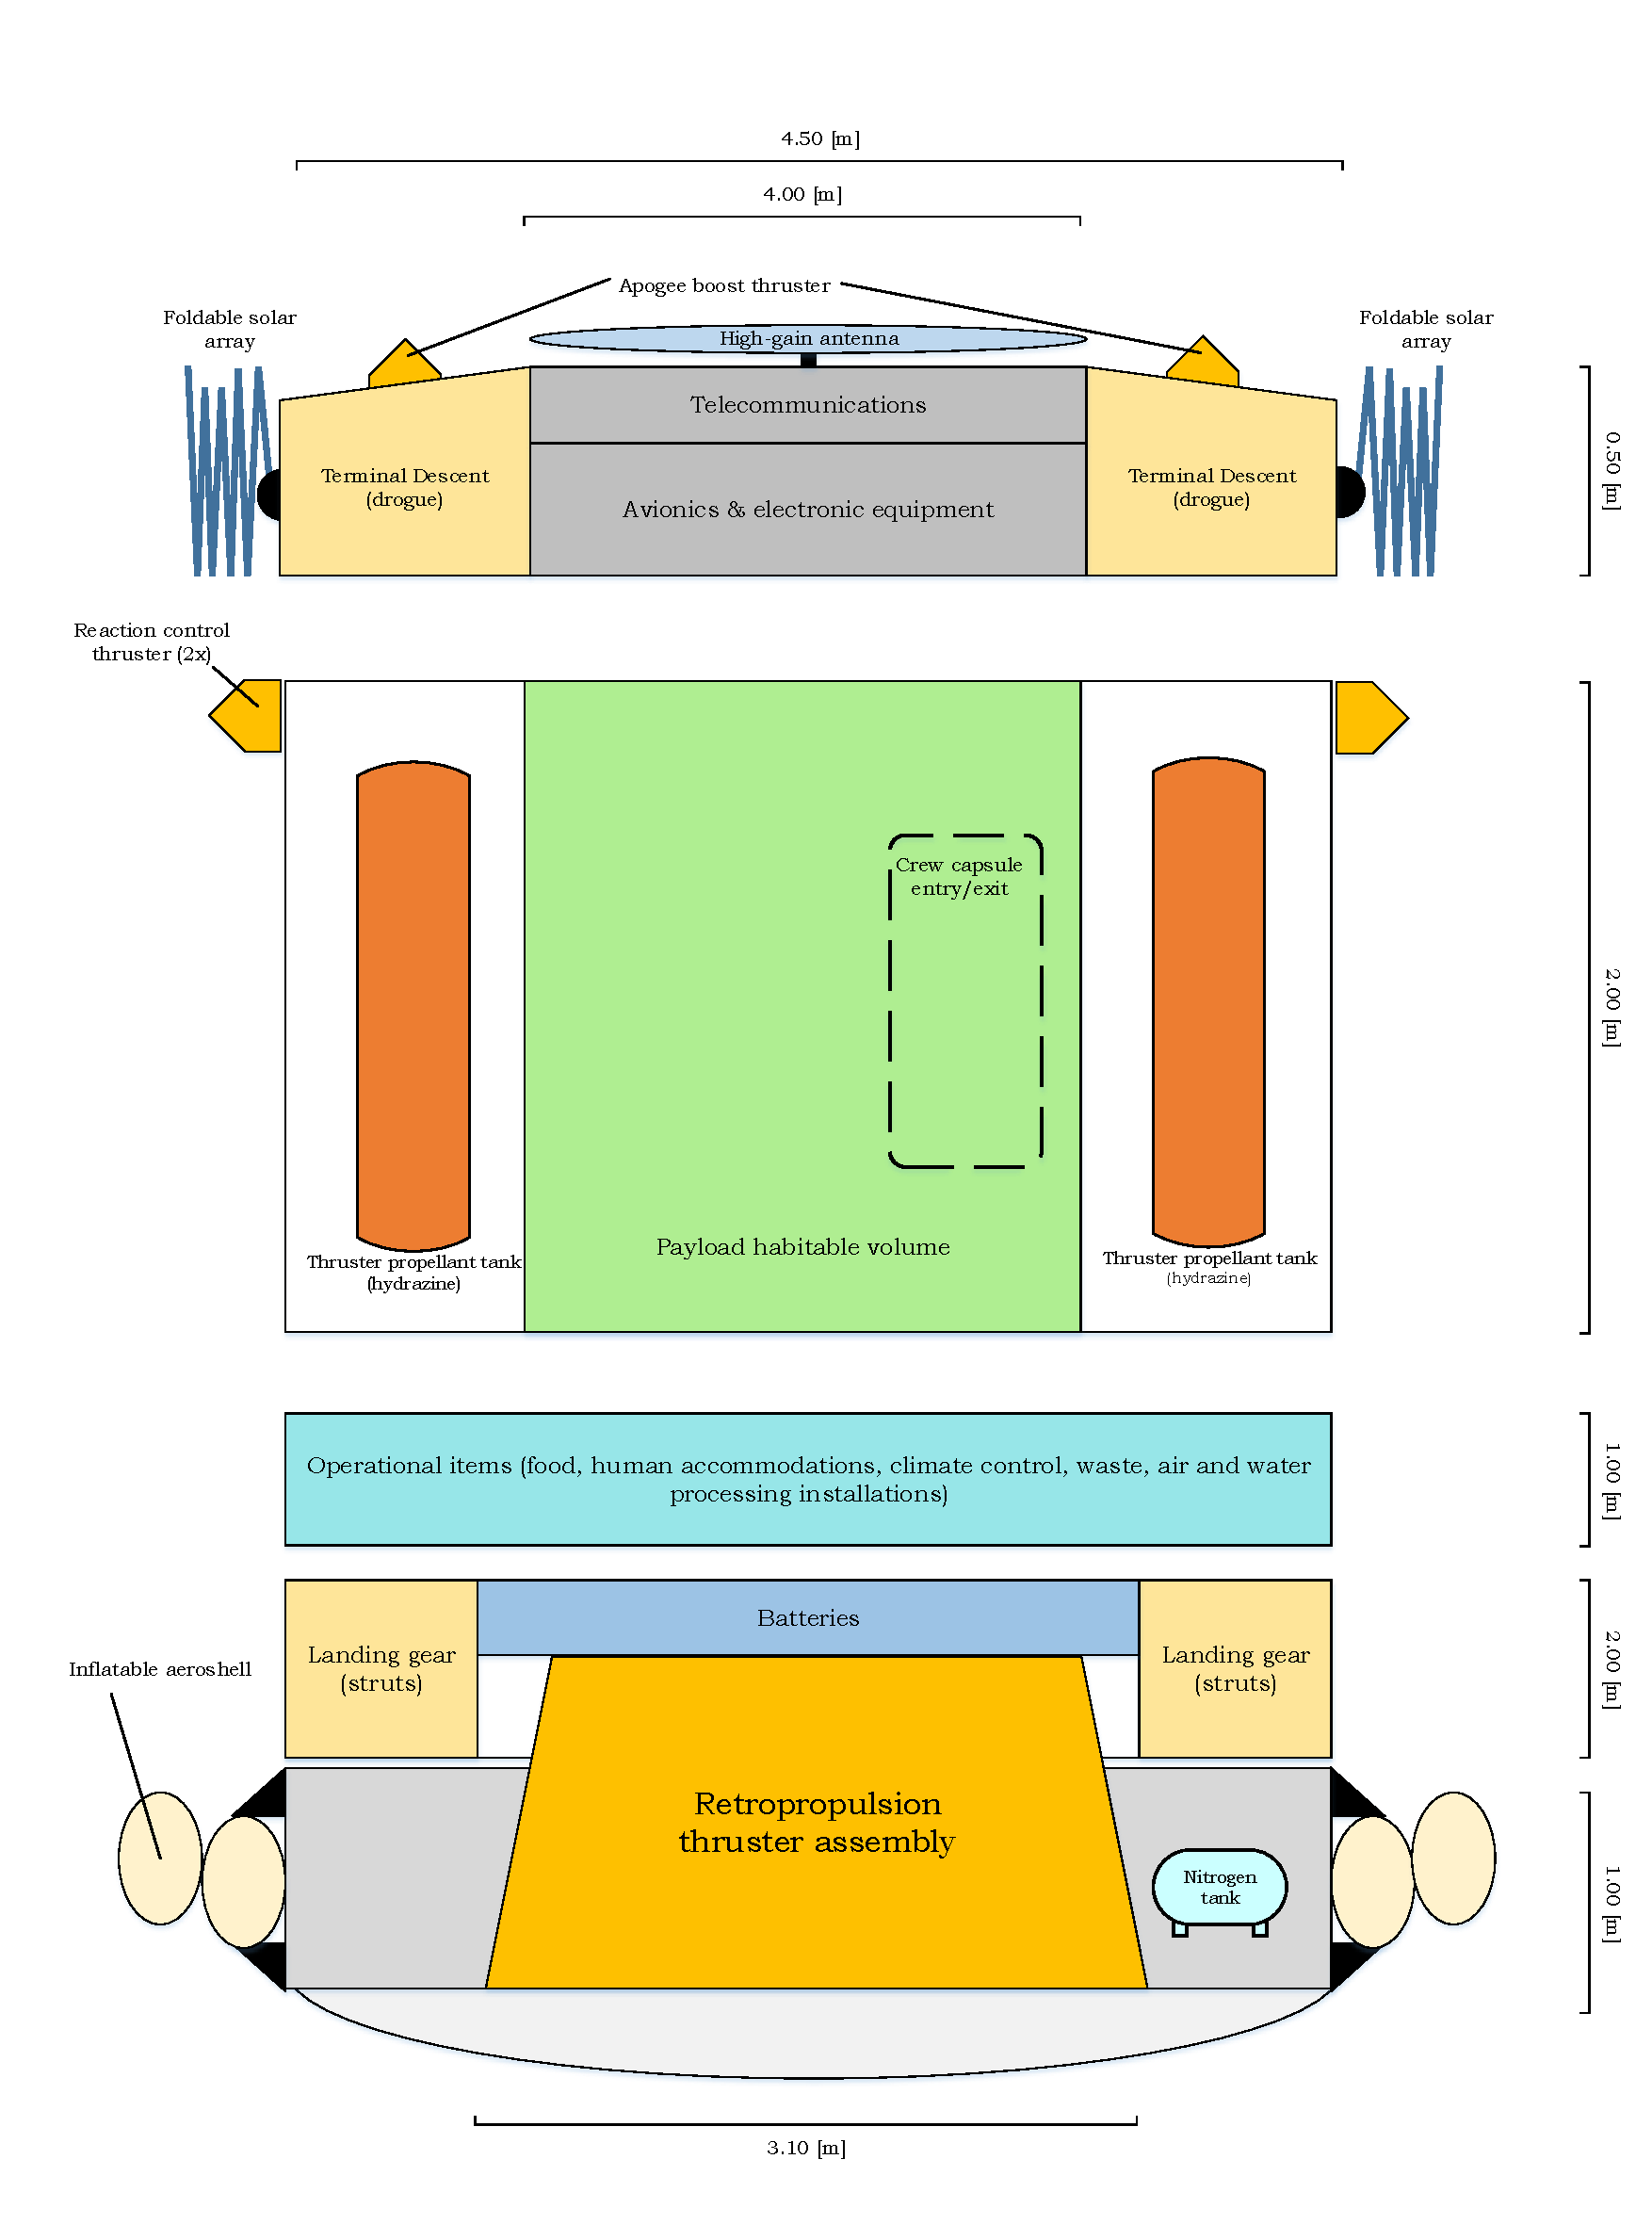
\includegraphics[width=0.95\textwidth]{./Figure/CrewModule/Axialview.pdf}
		\caption{Axial view of crew module lay-out}
		\label{fig:axview}
\end{figure}

\begin{figure}[h]
		\centering
		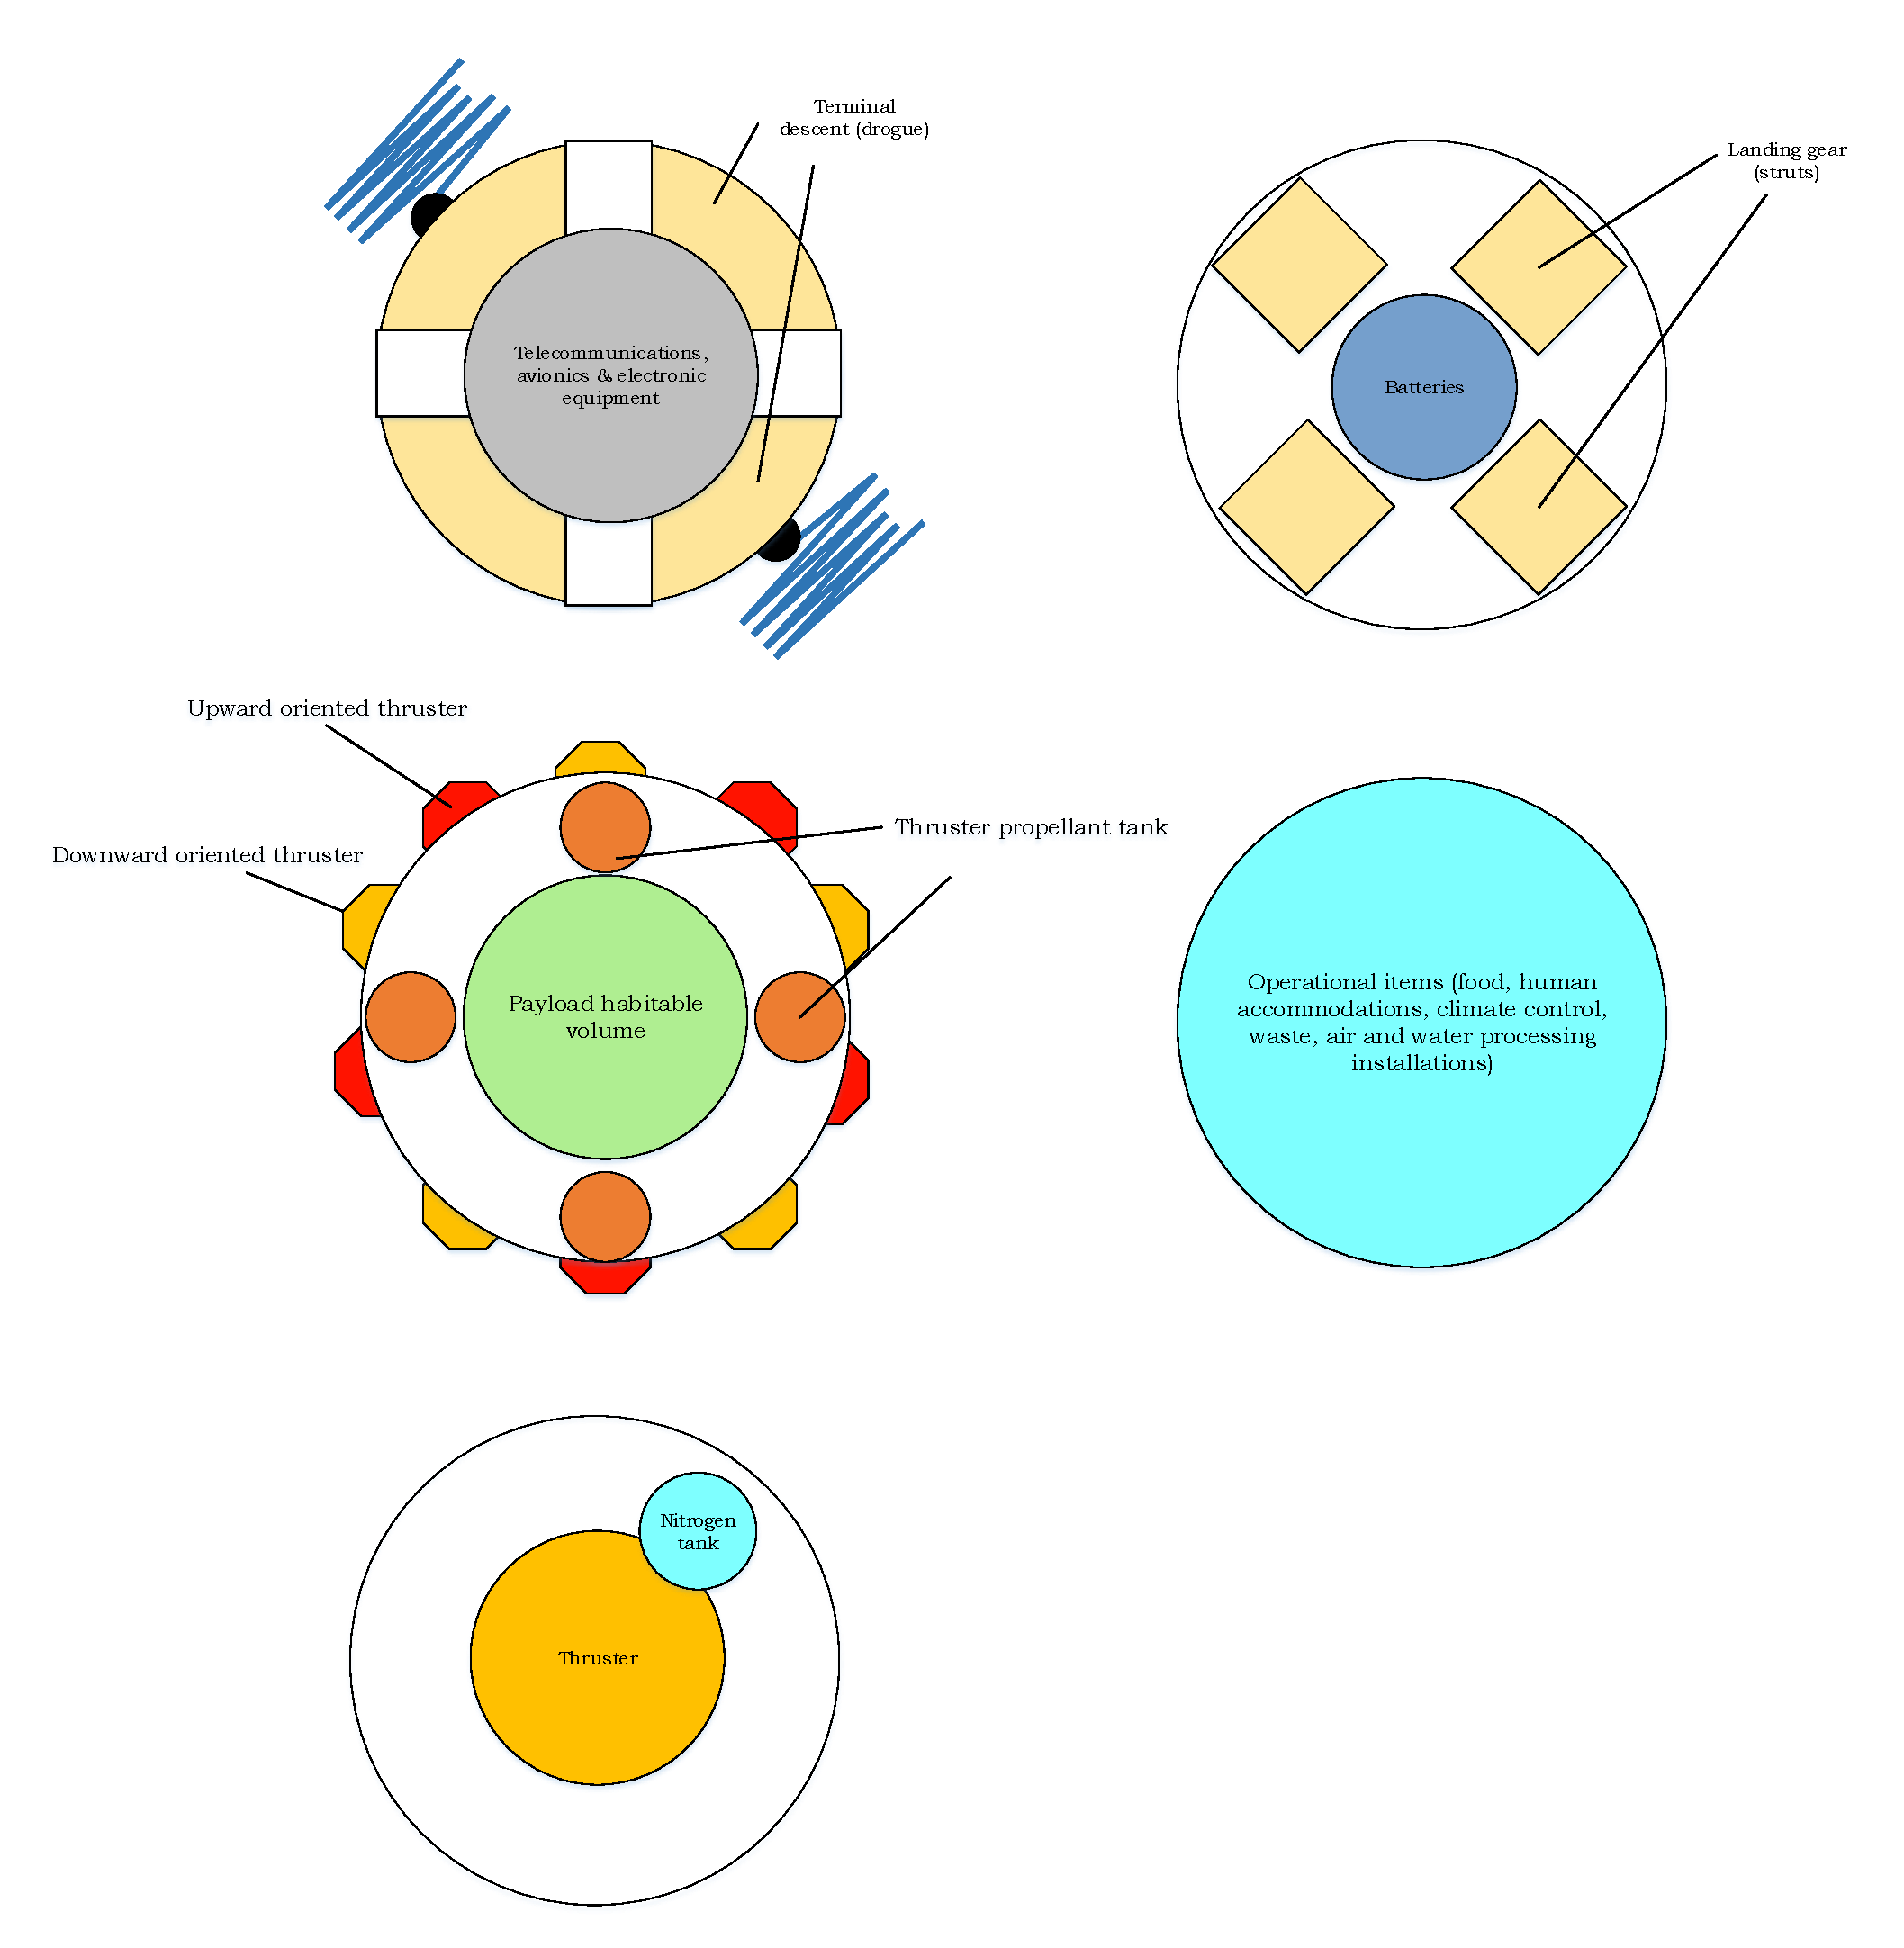
\includegraphics[width=0.95\textwidth]{./Figure/CrewModule/TopviewV2.pdf}
		\caption{Top-down view of crew module lay-out}
		\label{fig:topview}
\end{figure}


